\chapter{Simulación}
En esta sección se presentarán las simulaciones realizadas a través de LTSpiceXVII para medir los parámetros 
característicos del Darlington tanto con carga activa como carga pasiva. Por otro lado, también se desarrollará 
un análisis de Montecarlo para poder observar las sensibilidades del circuito.


\section{Circuito de Polarización}

\subsection{Carga Pasiva}

Primeramente, se realizó la simulación para la polarización del circuito con una carga pasiva de $R_E$ = $900 \Omega$.
\begin{figure}[H]
    \centering
    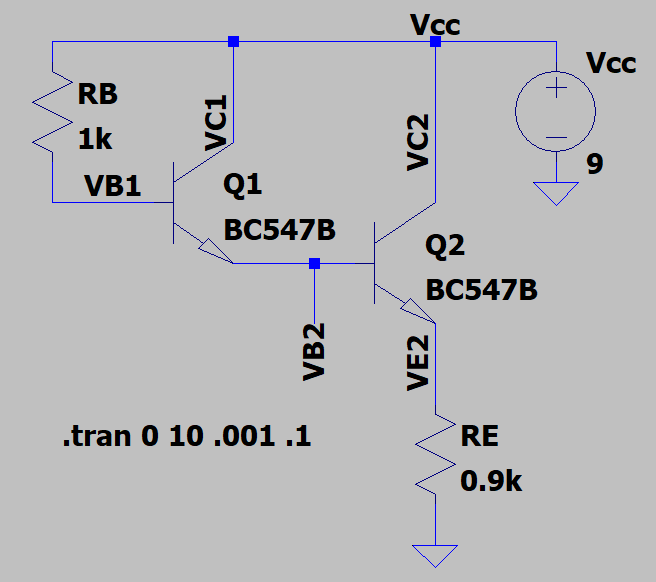
\includegraphics[width=0.35\textwidth]{3_simulacion/fig/circuito_pol_pas.png}
    \label{circuito_pol_pas}
    \caption{Circuito de Polarización configurado en LTSpiceXVII}
\end{figure}

Se obtuvieron los siguientes valores:

\begin{figure}[H]
    \centering
    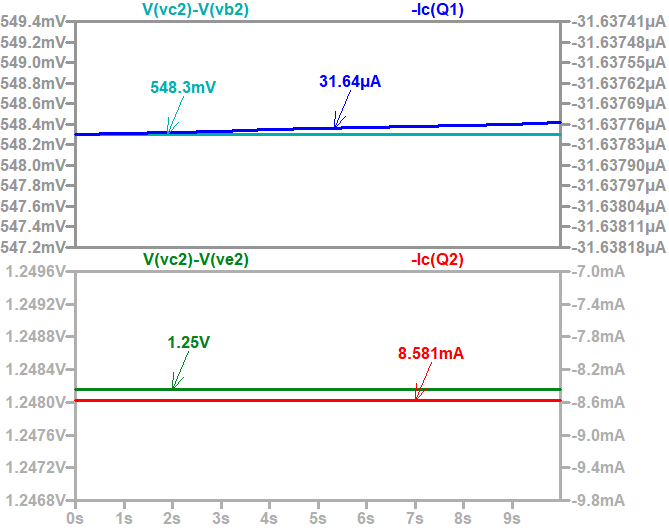
\includegraphics[width=0.5\textwidth]{3_simulacion/fig/pol_pasiva.png}
    \label{mediciones_pol_pas}
    \caption{Mediciones - Circuito de polarización con carga pasiva}
\end{figure}

A continuación, se presenta una tabla con las diferencias entre el modelo teórico y simulado:

\begin{table}[H]
    \centering
    \begin{tabular}{|c|c|c|c|}
    \hline
                        & Teórico & Simulado & Error[\%] \\ \hline
    $V_{CE1}[V]$        & $0.6$   & $0.583$  & $2.9$    \\ \hline
    $V_{CE2}[V]$        & $1.2$   & $1.25$   & $4.16$   \\ \hline
    $I_{CQ1}[\mu A]$ & $29.6$  & $31.64$  & $6.89$   \\ \hline  
    $I_{CQ2}[mA]$ & $8.64$  & $8.58$  & $0.69$   \\ \hline
    \end{tabular}
    \end{table}


\subsection{Carga Activa}

Luego, se calculó  para la polarización del circuito con una carga activa implementada con un espejo de corriente.

\begin{figure}[H]
    \centering
    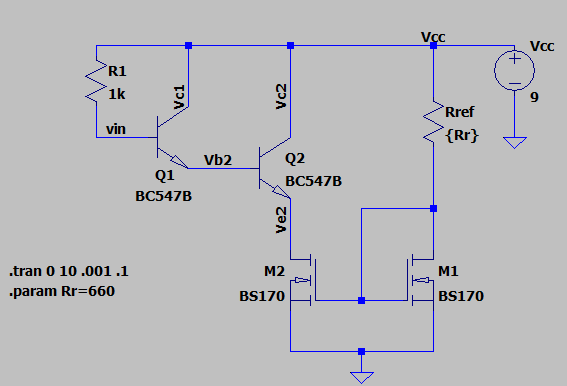
\includegraphics[width=0.35\textwidth]{3_simulacion/fig/circuito_pol_act.png}
    \label{circuito_pol_activa}
    \caption{Circuito de Polarización configurado en LTSpiceXVII}
\end{figure}

Se obtuvieron los siguientes valores:

\begin{figure}[H]
    \centering
    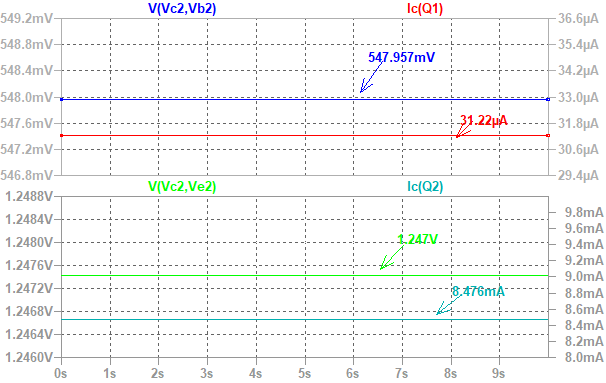
\includegraphics[width=0.5\textwidth]{3_simulacion/fig/pol_activa.png}
    \label{mediciones_pol_activa}
    \caption{Mediciones - Circuito de polarización con carga activa}
\end{figure}

A continuación, se presenta una tabla con las diferencias entre el modelo teórico y simulado:

\begin{table}[H]
    \centering
    \begin{tabular}{|c|c|c|c|}
    \hline
                        & Teórico & Simulado & Error[\%] \\ \hline
    $V_{CE1}[V]$        & $0.6$   & $0.547$  & $9.68$    \\ \hline
    $V_{CE2}[V]$        & $1.2$   & $1.247$   & $3.91$   \\ \hline
    $I_{CQ1}[\mu A]$ & $29.6$  & $31.22$  & $5.47$   \\ \hline
    $I_{CQ2}[mA]$ & $8.64$  & $8.48$  & $1.88$   \\ \hline
    \end{tabular}
    \end{table}



\section{Parámetros de Pequeña Señal}
Los parámetros de pequeña señal obtenidos con las mediciones se presentan en la siguiente tabla:

\begin{table}[H]
    \centering
    \begin{tabular}{|l|r|r|r|r|}
        \hline
        \multirow{2}{*}{} & \multicolumn{2}{c|}{Carga Pasiva} & \multicolumn{2}{c|}{Carga Activa} \\ \cline{2-5} 
         & $Q_1$ & $Q_2$ & $Q_1$ & $Q_2$ \\ \hline
        $h_{ie} (\si{\kilo\ohm})$ & $121.69$ & $0.488$ & $123.33$ & $0.454$ \\
        $h_{oe} (\si{\micro\siemens})$ & $0.527$ & $143$ & $0.520$ & $141.33$ \\\hline
    \end{tabular}
    \caption{Valores  obtenidos en base a simulación}
    \label{tab:vals_teo_2}
\end{table}

\section{Circuito Incremental}
El siguiente paso será realizar el circuito incremental del circuito desde el cual podremos obtener diversos parámetros 
característicos de nuestro circuito. Posteriormente, se presenta un estudio de Montecarlo para ver el efecto de 
las sensibilidades.

\begin{figure}[H]
    \centering
    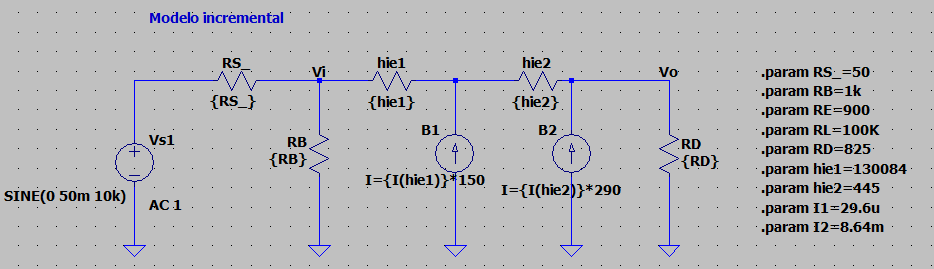
\includegraphics[width=0.95\textwidth]{3_simulacion/fig/modelo_incremental.png}
    \label{mediciones_pol_activa}
    \caption{Modelo incremental implementado}
\end{figure}

\subsection{Ganancia de Tensión}

Para un circuito con carga pasiva se obtuvo la siguiente ganancia de tensión.

\begin{figure}[H]
    \centering
    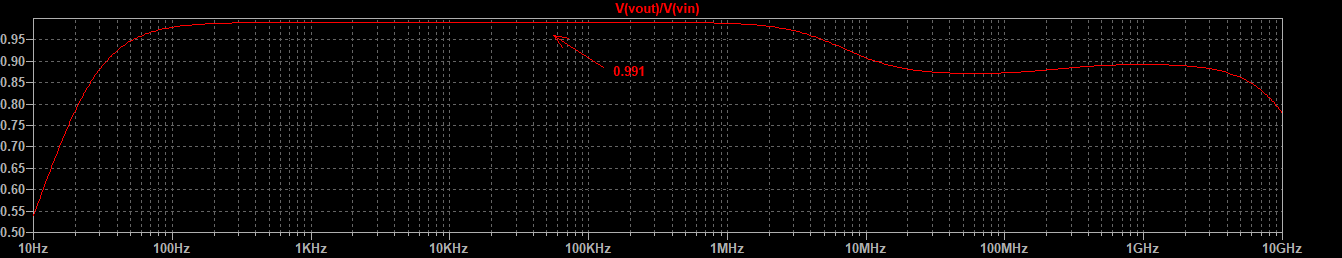
\includegraphics[width=0.95\textwidth]{3_simulacion/fig/ganancia_pasiva_ampli.png}
    \label{mediciones_pol_activa}
    \caption{Ganancia de tensión -  Carga pasiva}
\end{figure}

\begin{figure}[H]
    \centering
    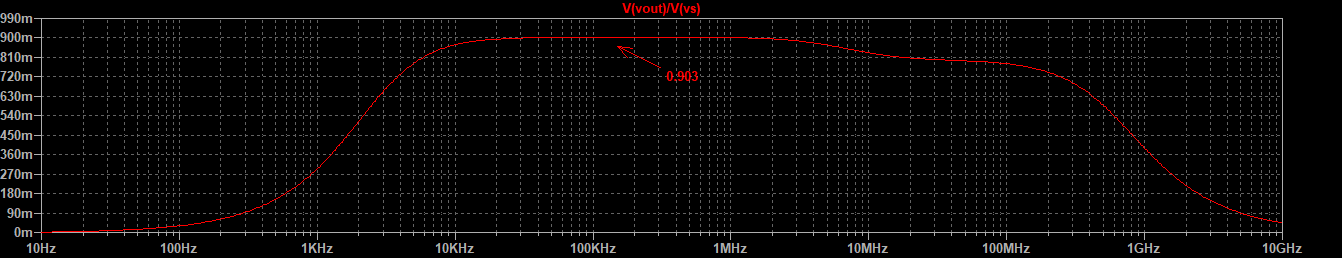
\includegraphics[width=0.95\textwidth]{3_simulacion/fig/ganancia_pasiva.png}
    \label{mediciones_pol_activa}
    \caption{Ganancia de tensión del sistema -  Carga pasiva}
\end{figure}

Esta es la primera simulación en la que se pudo ver reflejado el modelo visto en 
la materia respecto a la frecuencias medias, rango de validez asumido. En nuestra simulación,
dicho rango iría, según cierta rigurosidad, entre $10 KHz$ y $10 MHz$.

Se observa un error importante respecto a lo esperado para la ganancia de tensión del sistema, que debería ser según
estimaciones teóricas del orden de $0.95$. Este punto será revisado para la presentación.

Para un circuito con carga activa se obtuvo la siguiente ganancia de tensión.

\begin{figure}[H]
    \centering
    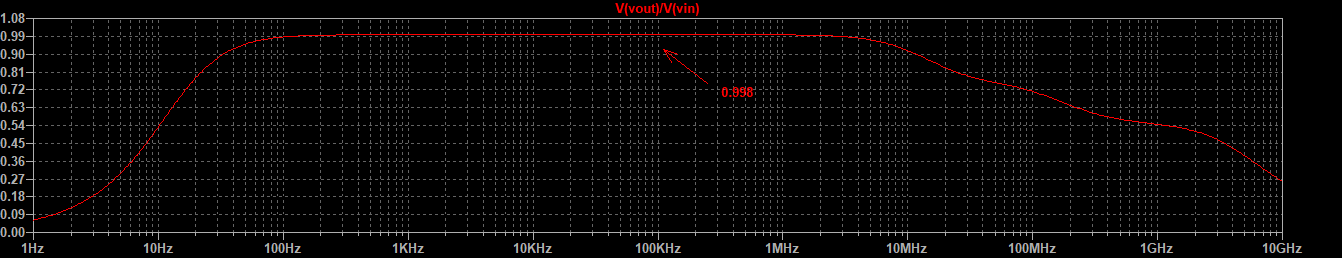
\includegraphics[width=0.95\textwidth]{3_simulacion/fig/ganancia_activa_ampli.png}
    \label{mediciones_pol_activa}
    \caption{Ganancia de tensión -  Carga activa}
\end{figure}

\begin{figure}[H]
    \centering
    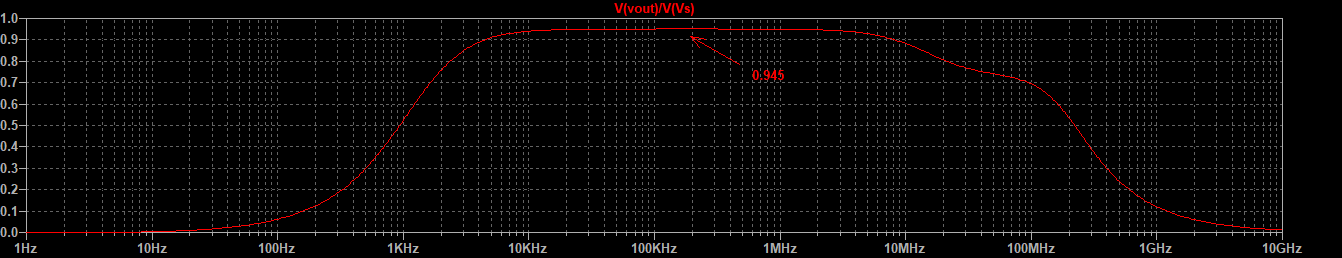
\includegraphics[width=0.95\textwidth]{3_simulacion/fig/ganancia_activa.png}
    \label{mediciones_pol_activa}
    \caption{Ganancia de tensión del sistema -  Carga activa}
\end{figure}

Las ganancias de tensión simuladas resultan ser similares a las esperadas según el desarrollo teórico.
\begin{table}[H]
    \centering
    \begin{tabular}{|c|c|c|}
    \hline
                        & Carga activa & Carga pasiva  \\ \hline
    $\Delta V$        & $0.998$   & $0.991$    \\ \hline
    $\Delta V_s$        & $0.945$   & $0.903$  \\ \hline
    \end{tabular}
    \end{table}


\subsection{Ganancia de Corriente}
Se realizó la simulación para obtener la ganancia de corriente.
\begin{figure}[H]
    \centering
    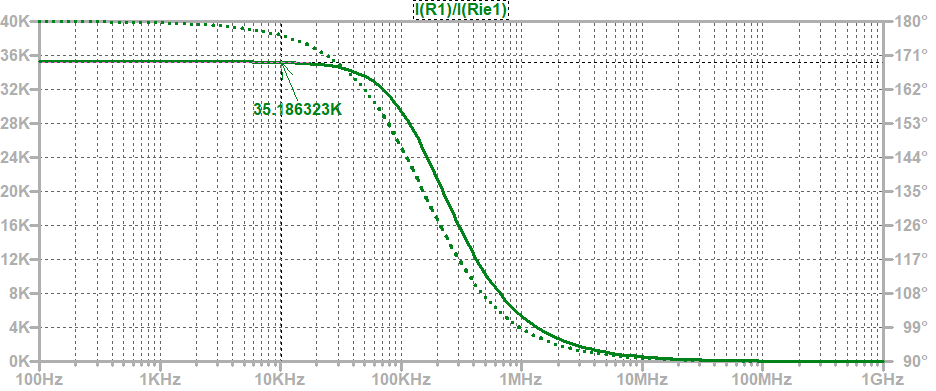
\includegraphics[width=0.75\textwidth]{3_simulacion/fig/tb1_Ai.png}
    \label{mediciones_pol_activa}
    \caption{Punto de operación del circuito en CC}
\end{figure}


\subsection{Impedancias de Entrada y Salida}
Primero, se buscó la impedancia de entrada para cada configuración.

\begin{figure}[H]
    \centering
    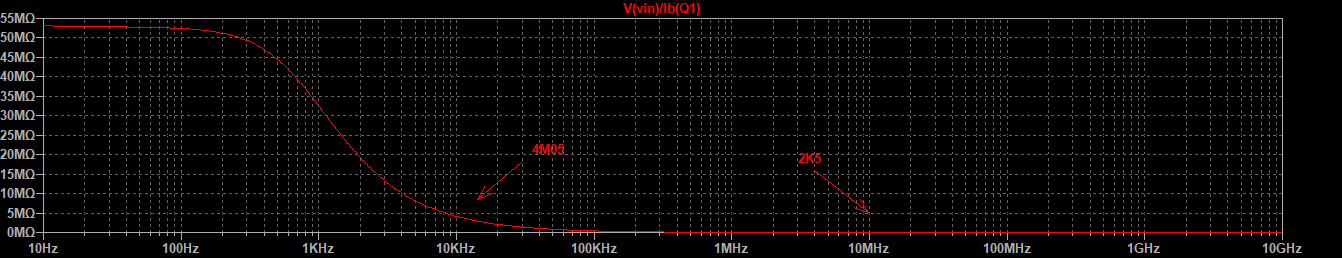
\includegraphics[width=0.75\textwidth]{3_simulacion/fig/impedancia_entrada_ampli_pasiva.png}
    \label{mediciones_pol_activa}
    \caption{Impedancia de entrada del amplificador - Carga pasiva}
\end{figure}

\begin{figure}[H]
    \centering
    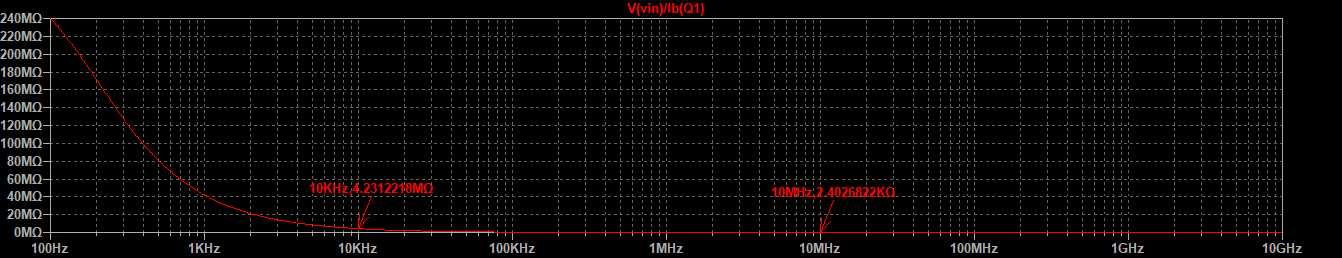
\includegraphics[width=0.75\textwidth]{3_simulacion/fig/impedancia_entrada_ampli_activa.png}
    \label{mediciones_pol_activa}
    \caption{Impedancia de entrada del amplificador - Carga activa}
\end{figure}

Luego, se calculó la impedancia de entrada del amplificador.
\begin{figure}[H]
    \centering
    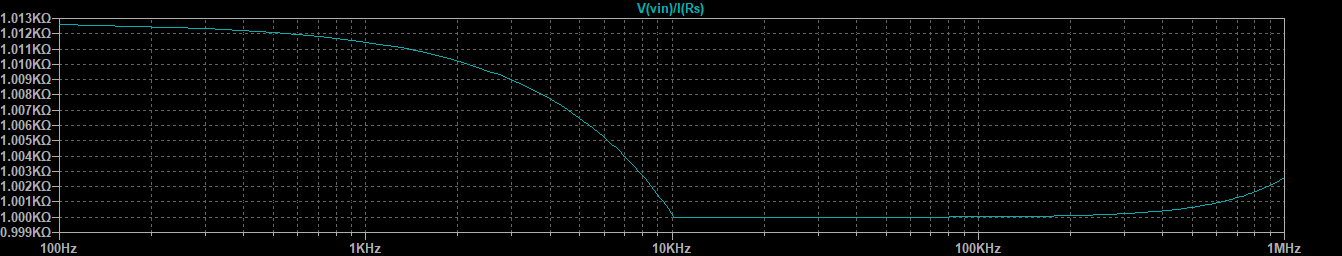
\includegraphics[width=0.75\textwidth]{3_simulacion/fig/rin.png}
    \label{mediciones_pol_activa}
    \caption{Impedancia de entrada del amplificador}
\end{figure}

La impedancia de entrada simulada fue consistente con la esperada ya que se obtuvo el valor de $R_B$,
tanto para carga activa como pasiva. Se observó una mínima variación antes de la zona de frecuencias medias. \par 


Para la impedancia de salida se realizó la siguiente simulación, pasivando las fuentes independientes 
y utilizando una tensión de prueba.

\begin{figure}[H]
    \centering
    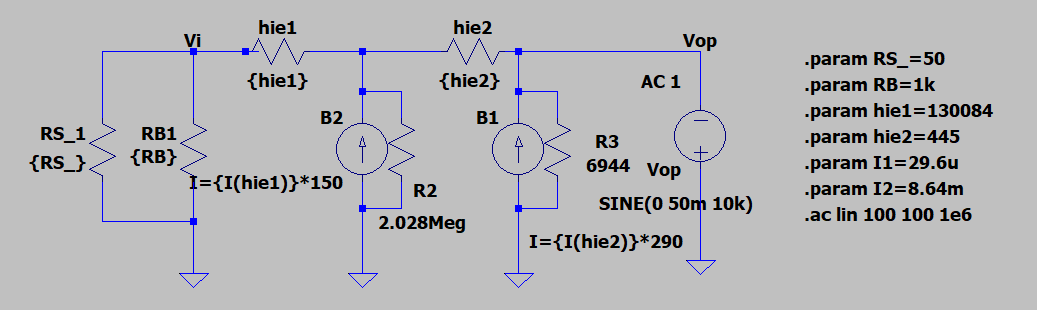
\includegraphics[width=0.75\textwidth]{3_simulacion/fig/circuito_ro.png}
    \label{mediciones_pol_activa}
    \caption{Mediciones - Circuito para medir impedancia de salida}
\end{figure}

De la misma se obtuvo el siguiente gráfico para la impedancia de salida en función de la frecuencia.

\begin{figure}[H]
    \centering
    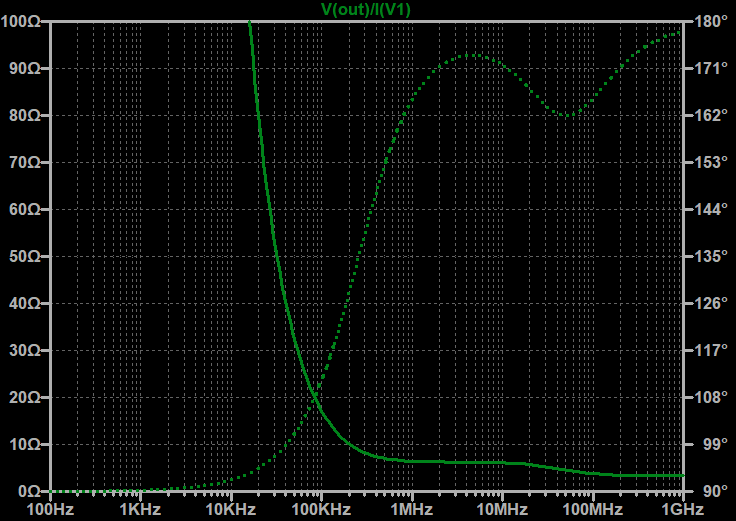
\includegraphics[width=0.5\textwidth]{3_simulacion/fig/ro.png}
    \label{mediciones_pol_activa}
    \caption{Impedancia de salida en función de la frecuencia}
\end{figure}

Como $r_o$ no depende de $R_E$ ni el equivalente de la fuente de corriente, se obtuvo lo mismo para ambas 
configuraciones. Se observó en la zona de frecuencias medias una impedancia de aproximadamente $6 \Omega$, 
consistente con lo expresado en la tabla [\ref{tab:vals_teo}].



\newpage
\section{Circuito Incremental}
Se simuló el comportamiento del circuito incremental primero con todos los componentes y como comparación con solo el modelo de pequeña señal.

\begin{figure}[ht]
    \centering
    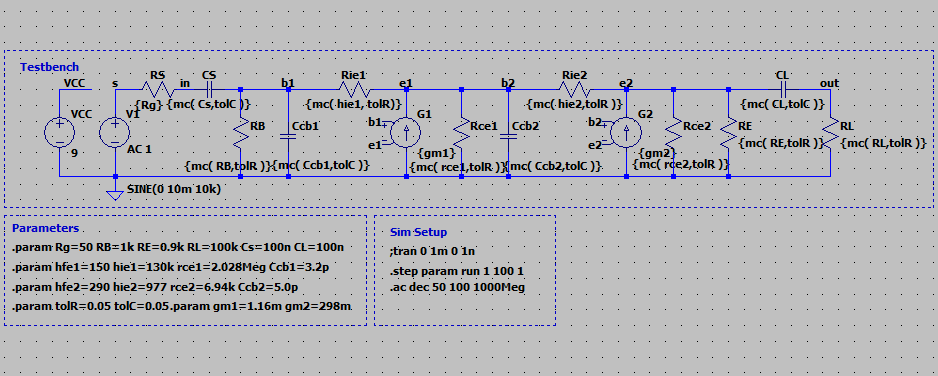
\includegraphics[width=\linewidth]{3_simulacion/fig/tb_1.png}
    \caption{Banco de prueba con modelo de pequeña señal}
\end{figure}

\begin{figure}[ht]
    \begin{minipage}[t]{0.48\textwidth}
        \centering
        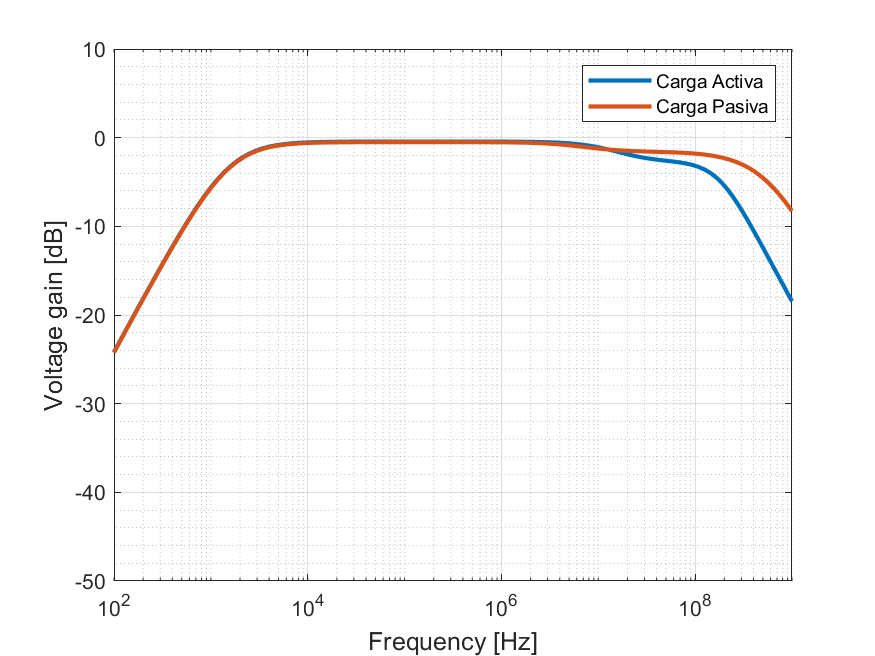
\includegraphics[width=\linewidth]{3_simulacion/fig/Bode_circuito.png}
        \caption{Respuesta en frecuencia de la ganancia de tensión de los circuitos}
        \label{fig:bode_cir}
    \end{minipage}\hfill
    \begin{minipage}[t]{0.48\textwidth}
        \centering
        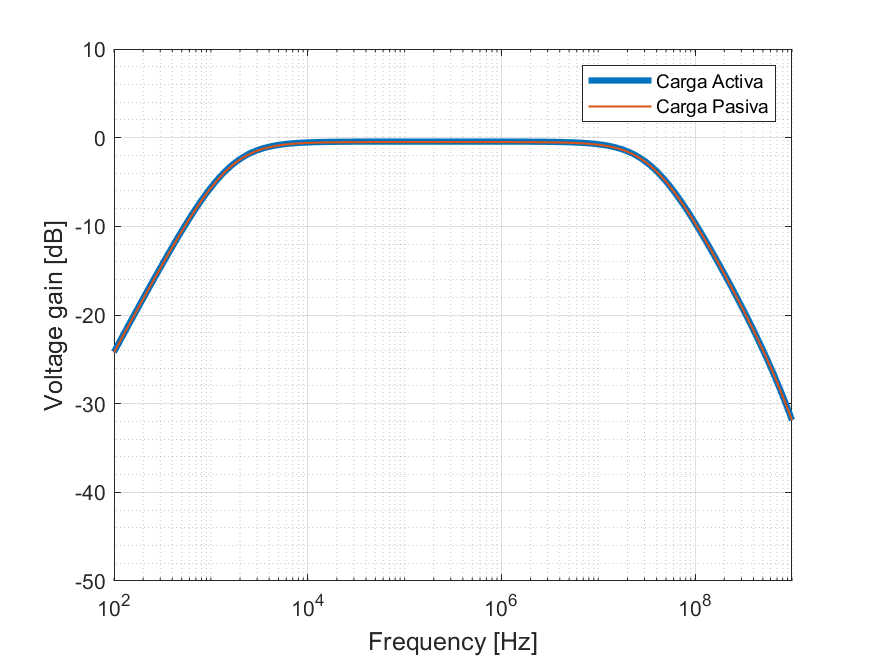
\includegraphics[width=\linewidth]{3_simulacion/fig/Bode_tb1.png}
        \caption{Respuesta en frecuencia de la ganancia de tensión del banco de prueba}
        \label{fig:bode_tb1}
    \end{minipage}
\end{figure}

Se puede observar una mejora en el circuito con carga activa al acortar el ancho de banda a altas frecuencias en la figura \ref{fig:bode_cir}. Por otro lado, hay una diferencia considerable entre la respuesta en frecuencia del circuito real y la del modelo incremental. Se encontró que esto ocurre por despreciar las capacitancias parásitas entre la base y el emisor.

Utilizando una nueva configuración donde se consideraron estas capacitancias, se obtuvo una simulación más acorde a la del circuito real (figura \ref{fig:bode_tb2}). Aún así, el circuito conserva su comportamiento de seguidor por emisor en las frecuencias medias.

Por último también se ejecutó el análisis de montecarlo para cada variación de los circuitos simulados. Se puede observar en cada caso cómo la aplicación de la carga activa en primer lugar acerca el polo dominante de alta frecuencia, reduciendo el ancho de banda.

\begin{figure}
    \centering
    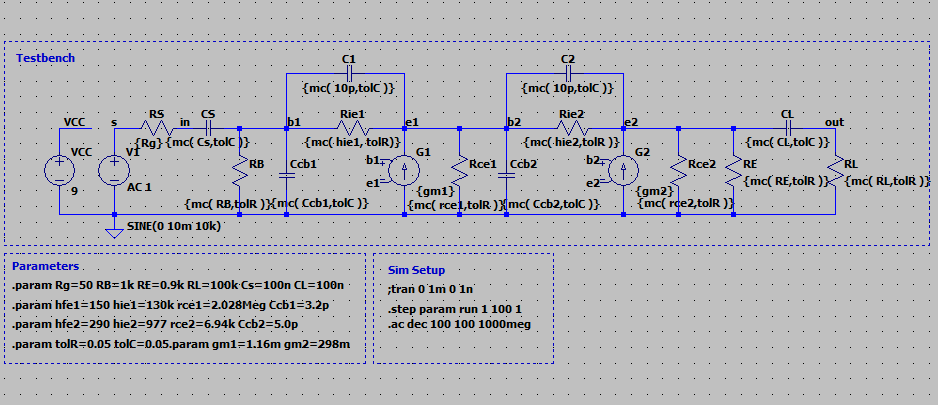
\includegraphics[width=\linewidth]{3_simulacion/fig/tb_2.png}
    \caption{Banco de pruebas con Capacitancias Base Emisor}
\end{figure}

\begin{figure}
    \centering
    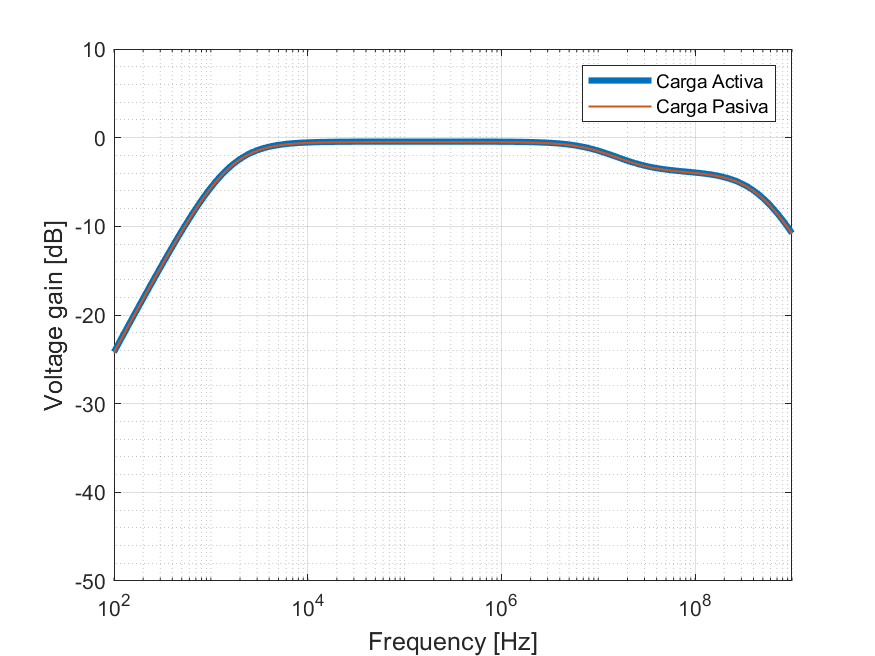
\includegraphics[width=0.5\linewidth]{3_simulacion/fig/Bode_tb2.png}
    \caption{Respuesta en frecuencia del banco de prueba con $C_{eb}$}
    \label{fig:bode_tb2}
\end{figure}

\begin{figure}
    \centering
    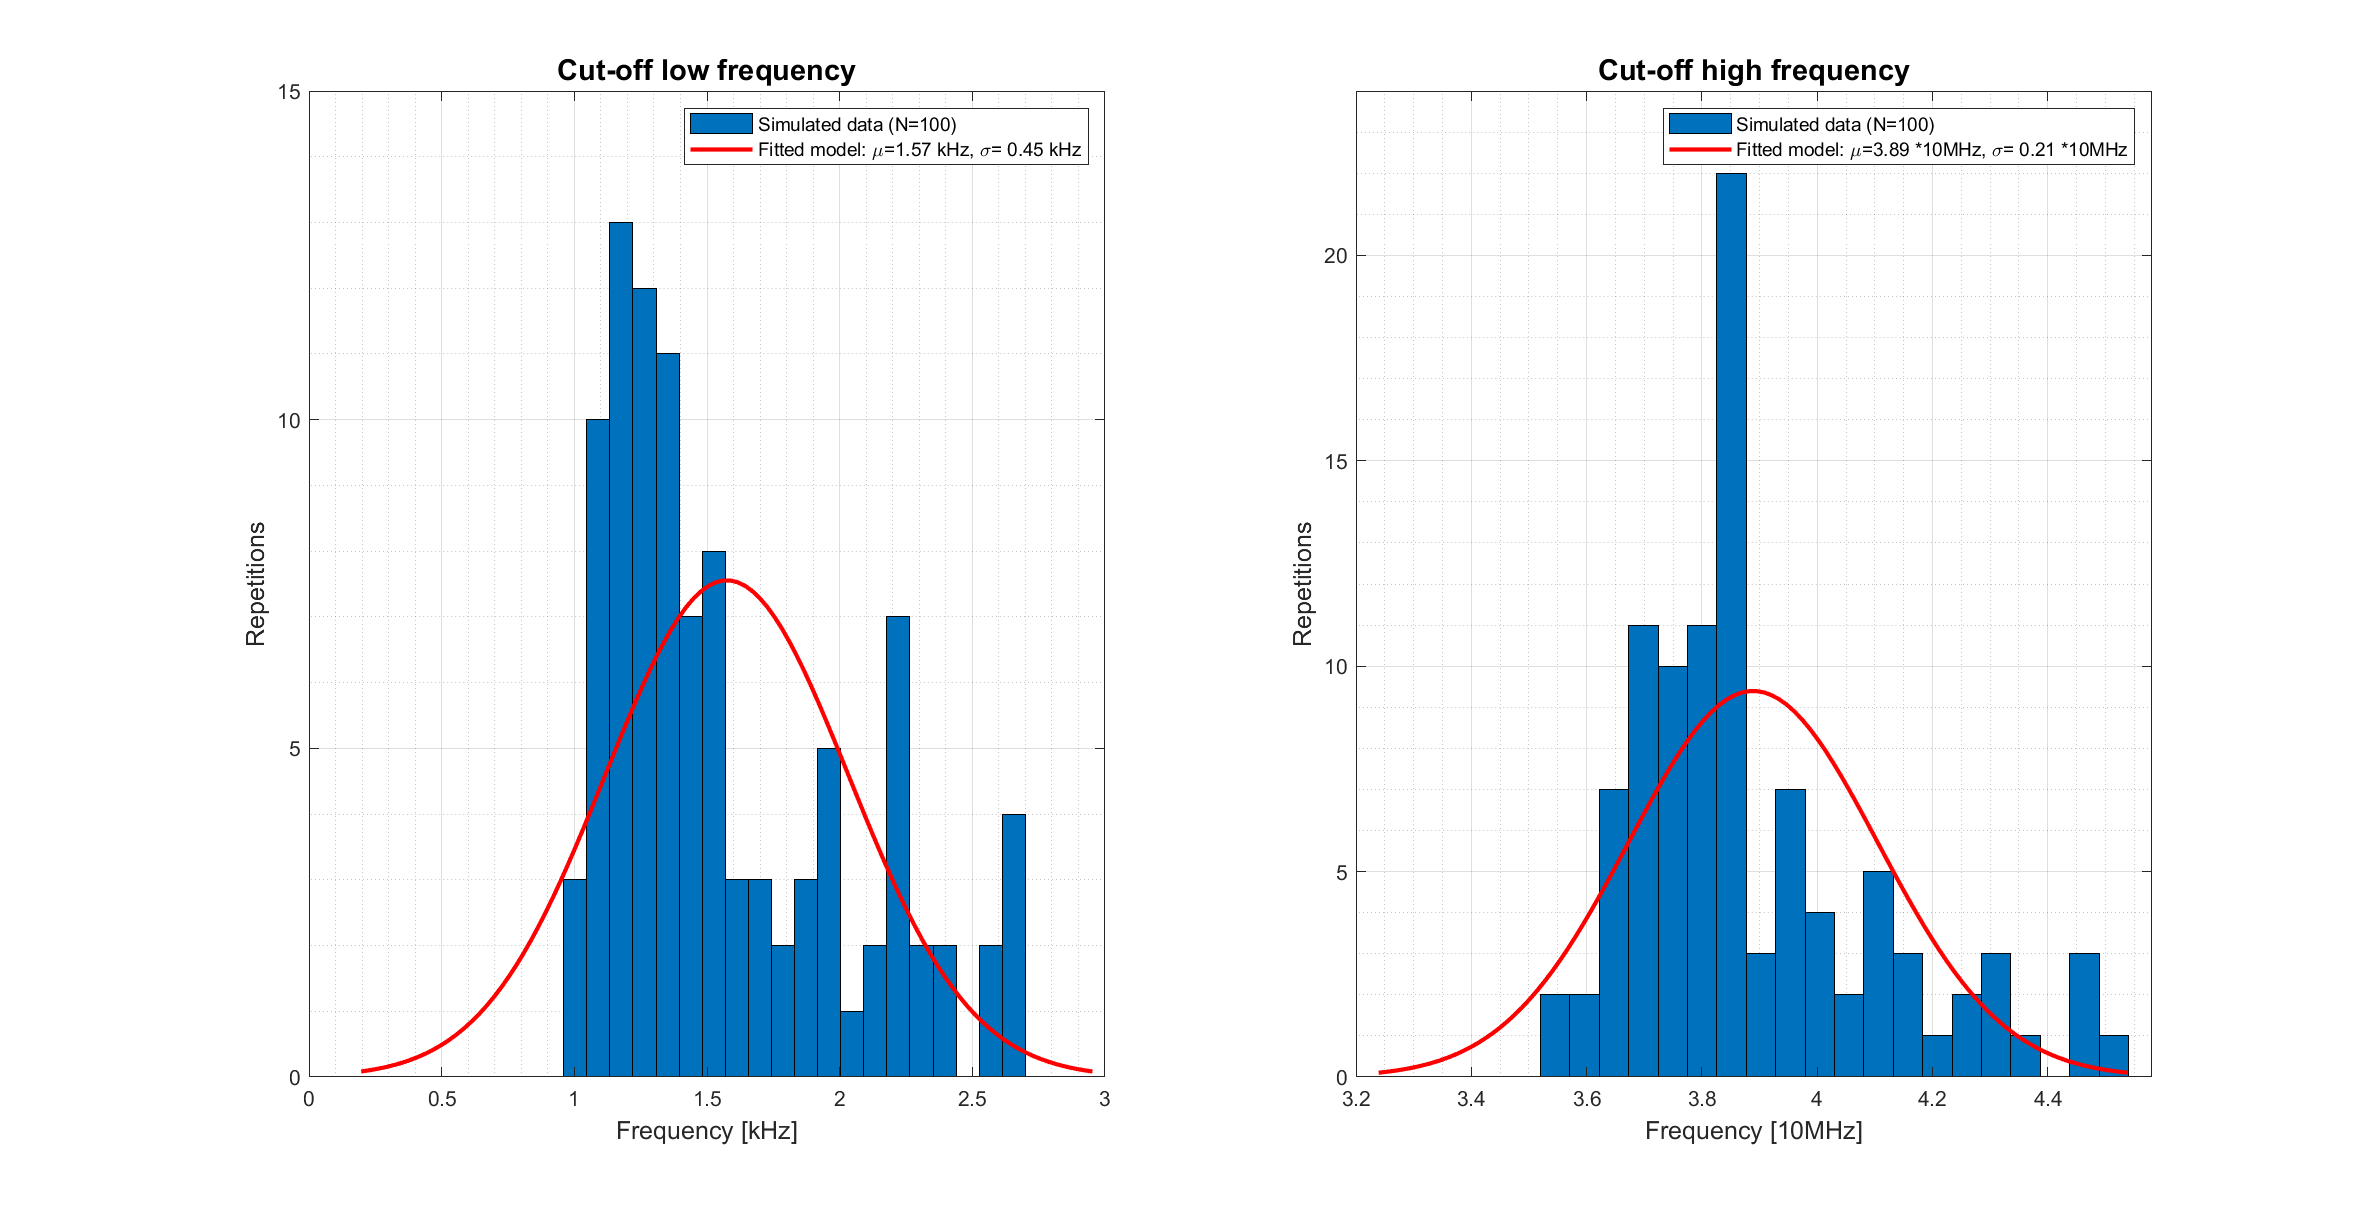
\includegraphics[width=\linewidth]{3_simulacion/fig/Hist_cir_pas_100.png}
    \caption{Análisis estadístico de los lugares de los polos de bajas y altas frecuencias con carga pasiva, circuito real}
\end{figure}

\begin{figure}
    \centering
    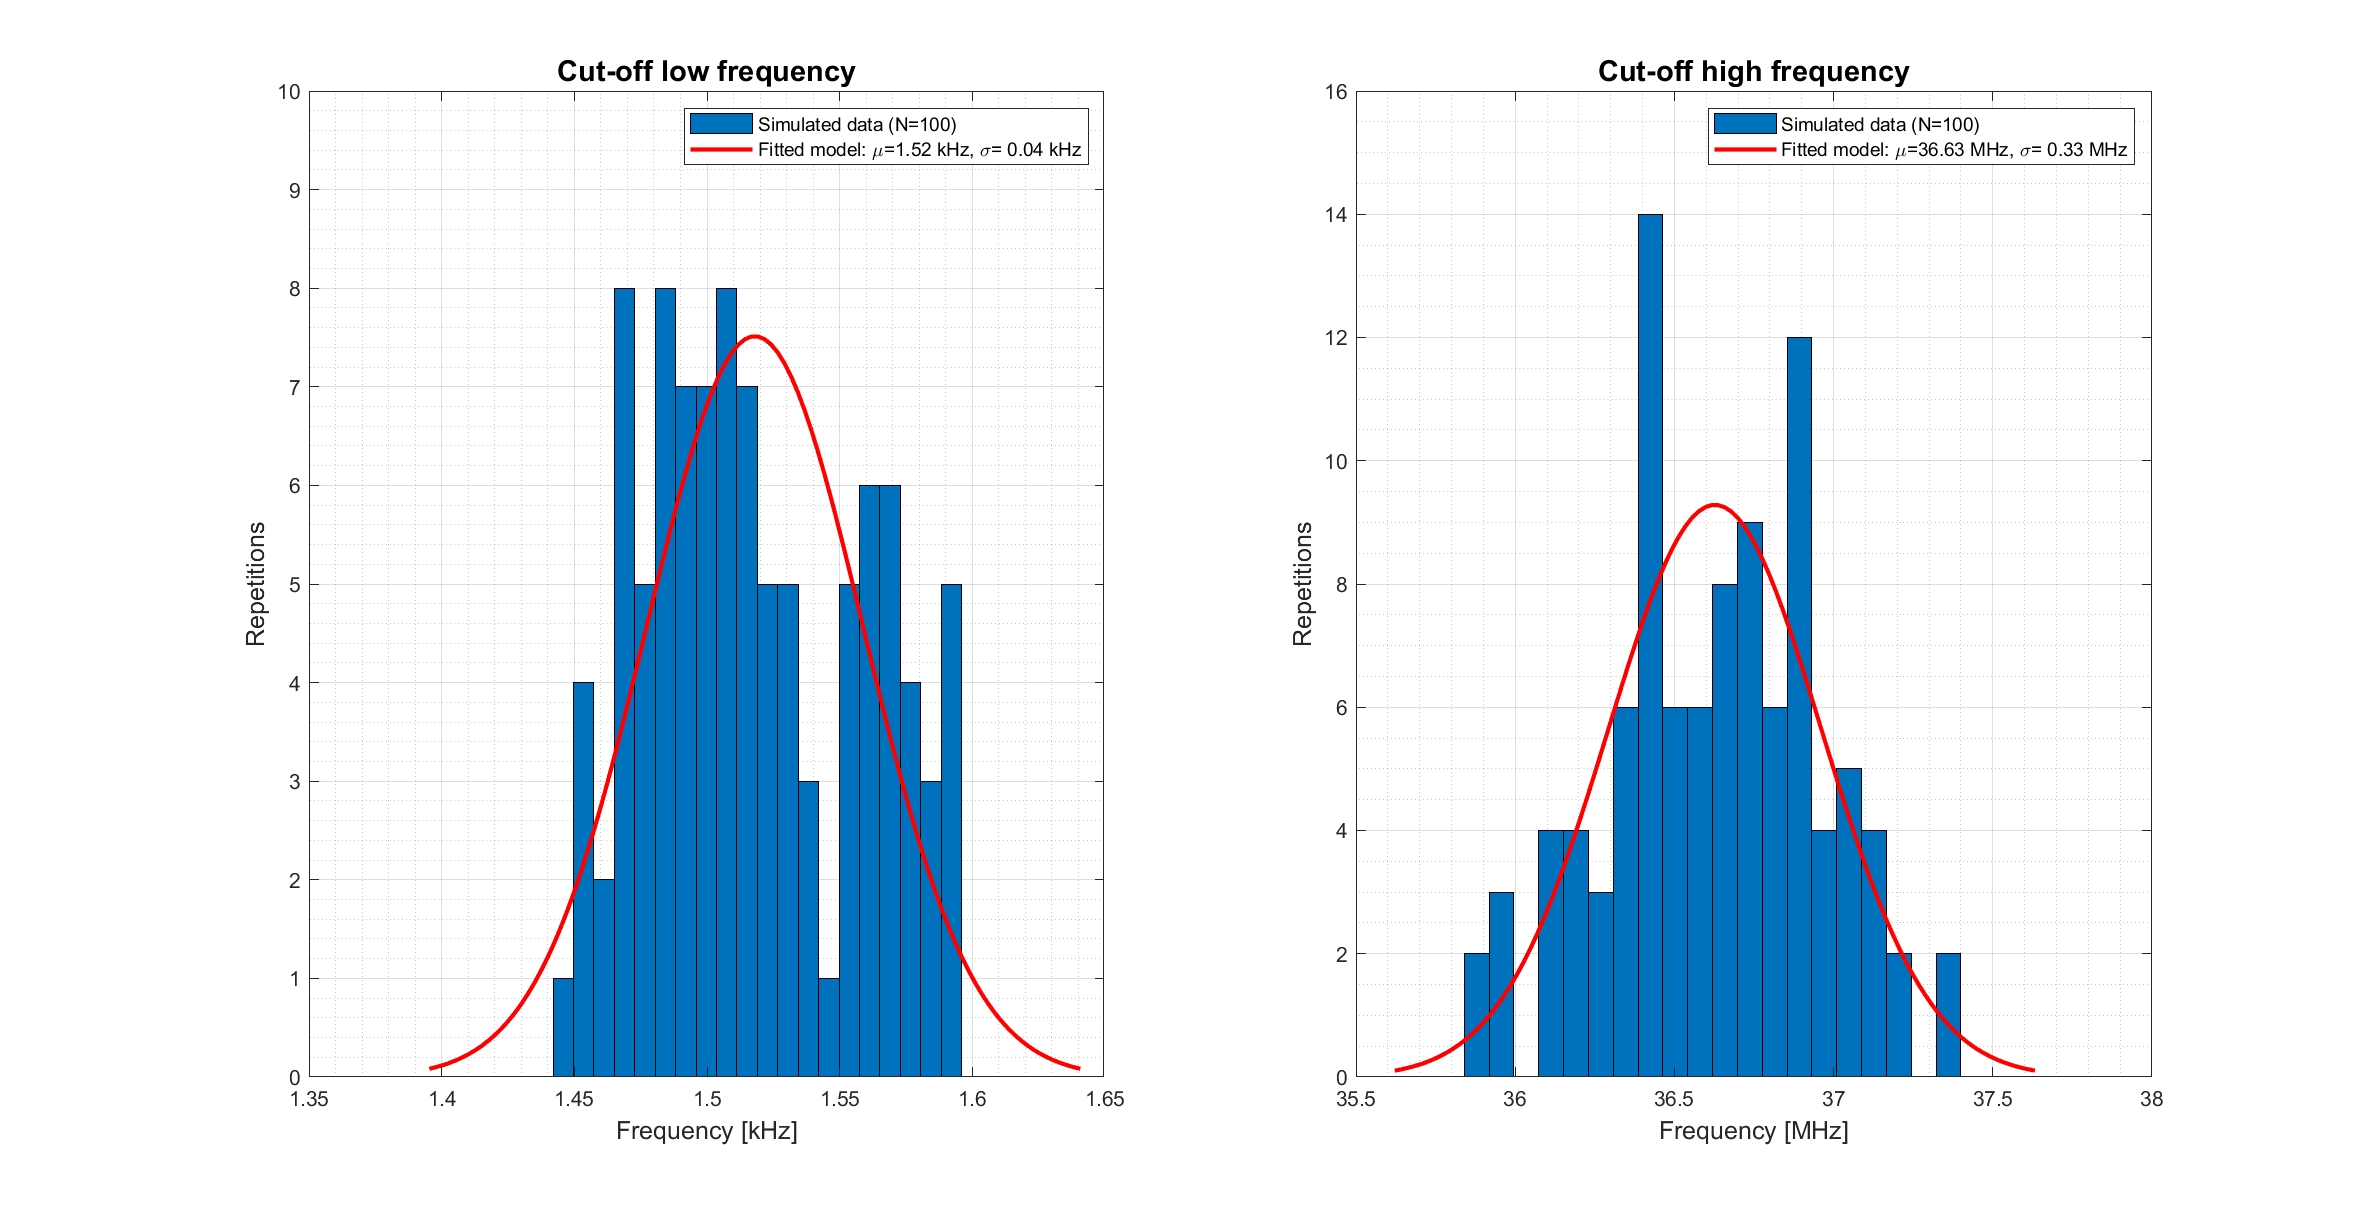
\includegraphics[width=\linewidth]{3_simulacion/fig/Hist_cir_act_100.png}
    \caption{Análisis estadístico de los lugares de los polos de bajas y altas frecuencias con carga activa, circuito real}
\end{figure}

\begin{figure}
    \centering
    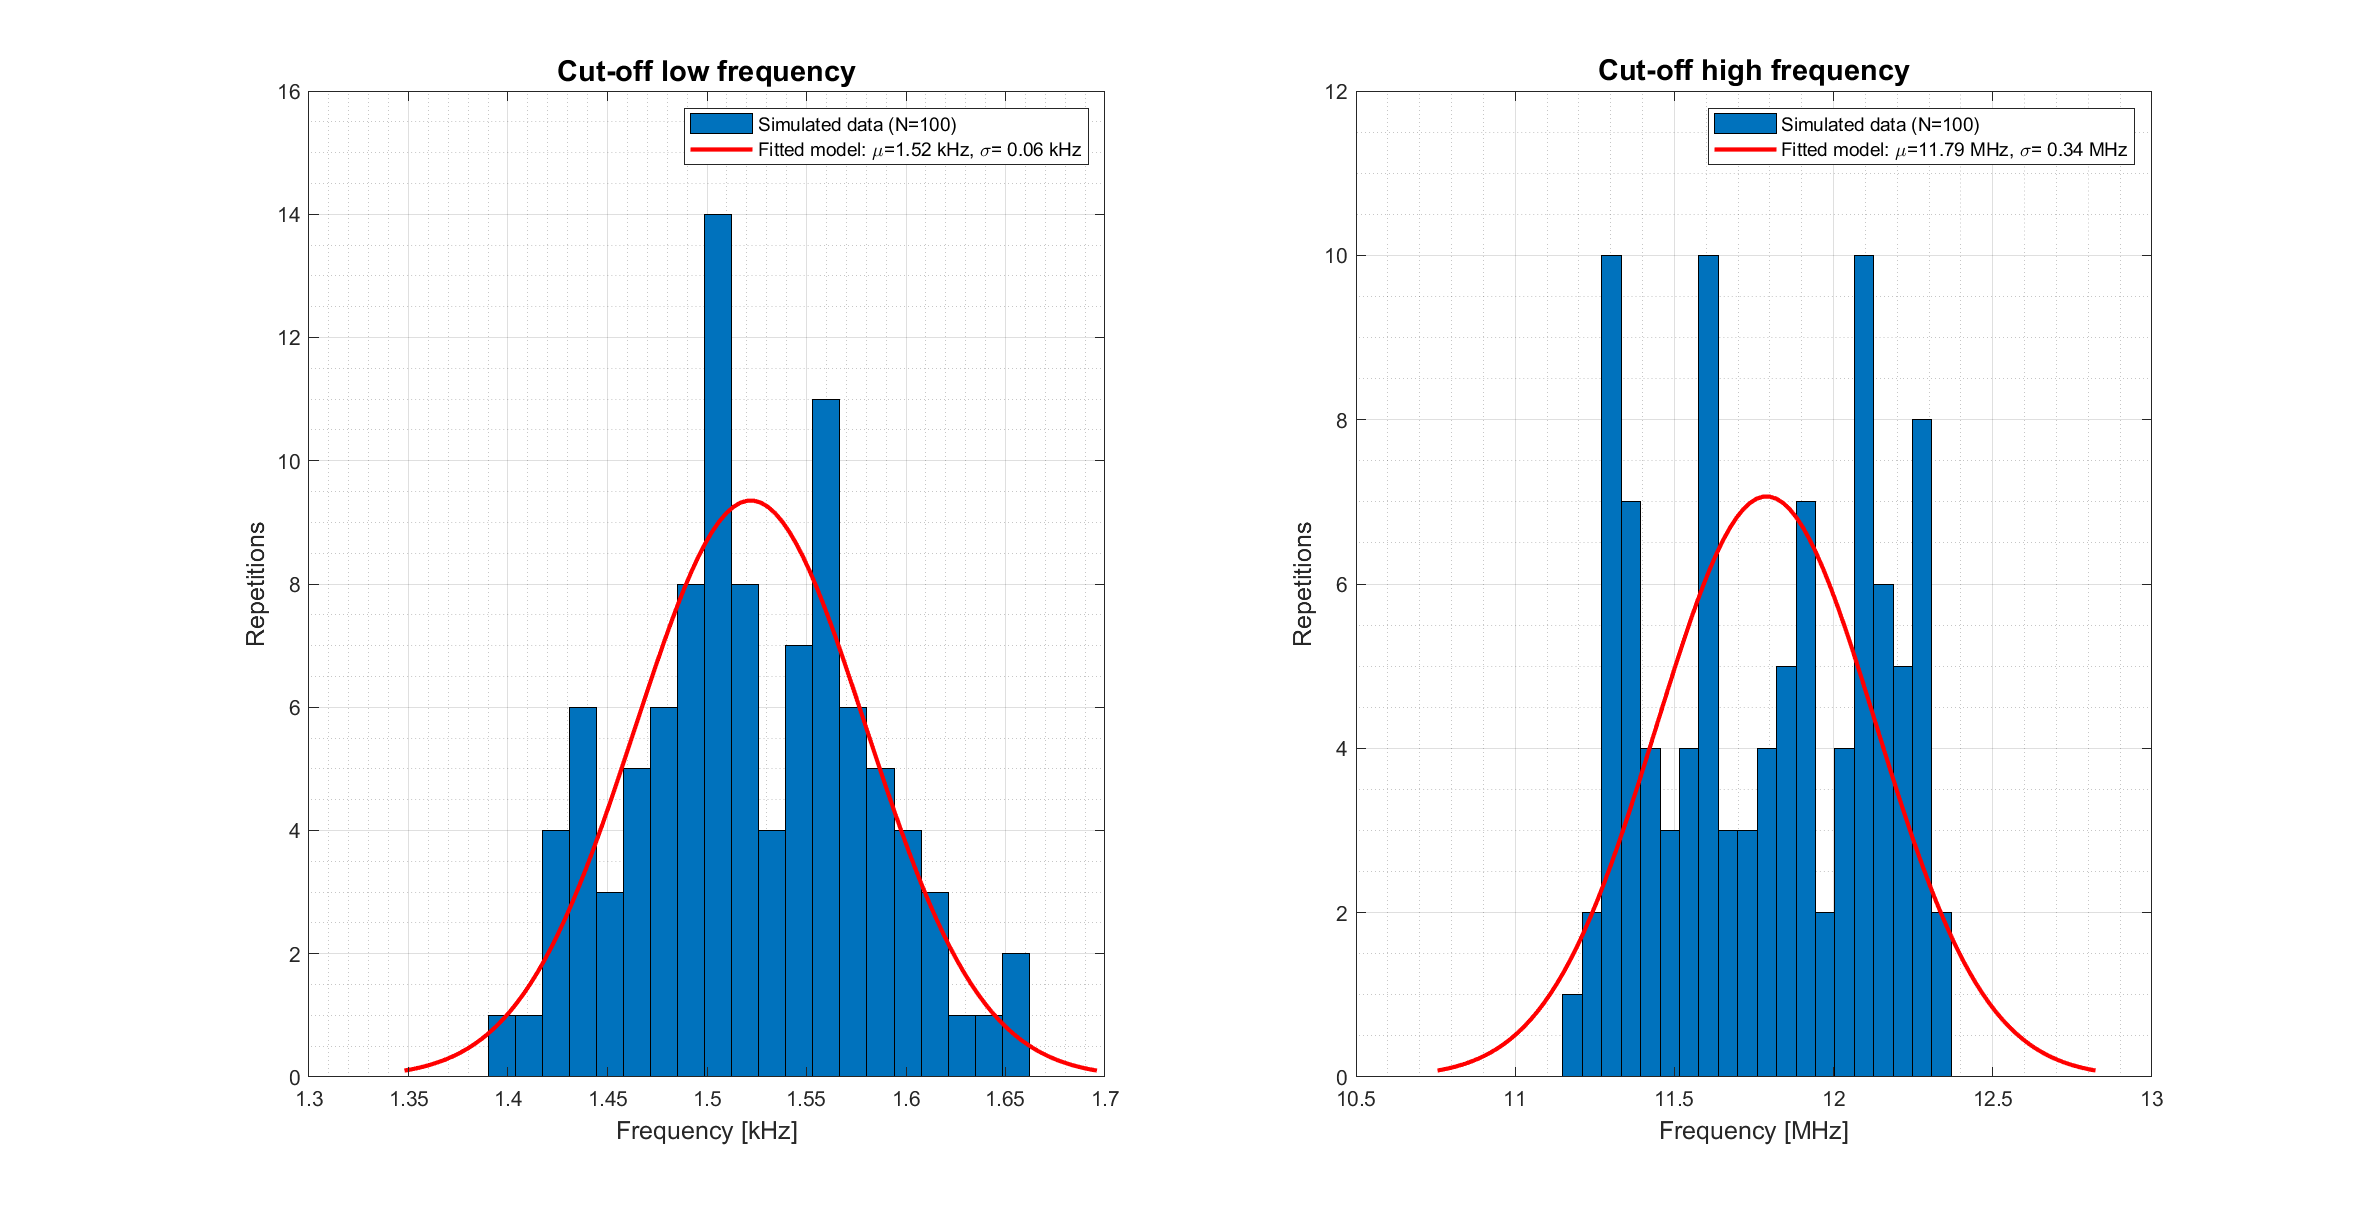
\includegraphics[width=\linewidth]{3_simulacion/fig/Hist_tb1_pas_100.png}
    \caption{Análisis estadístico de los lugares de los polos de bajas y altas frecuencias con carga pasiva, banco de pruebas 1}
\end{figure}

\begin{figure}
    \centering
    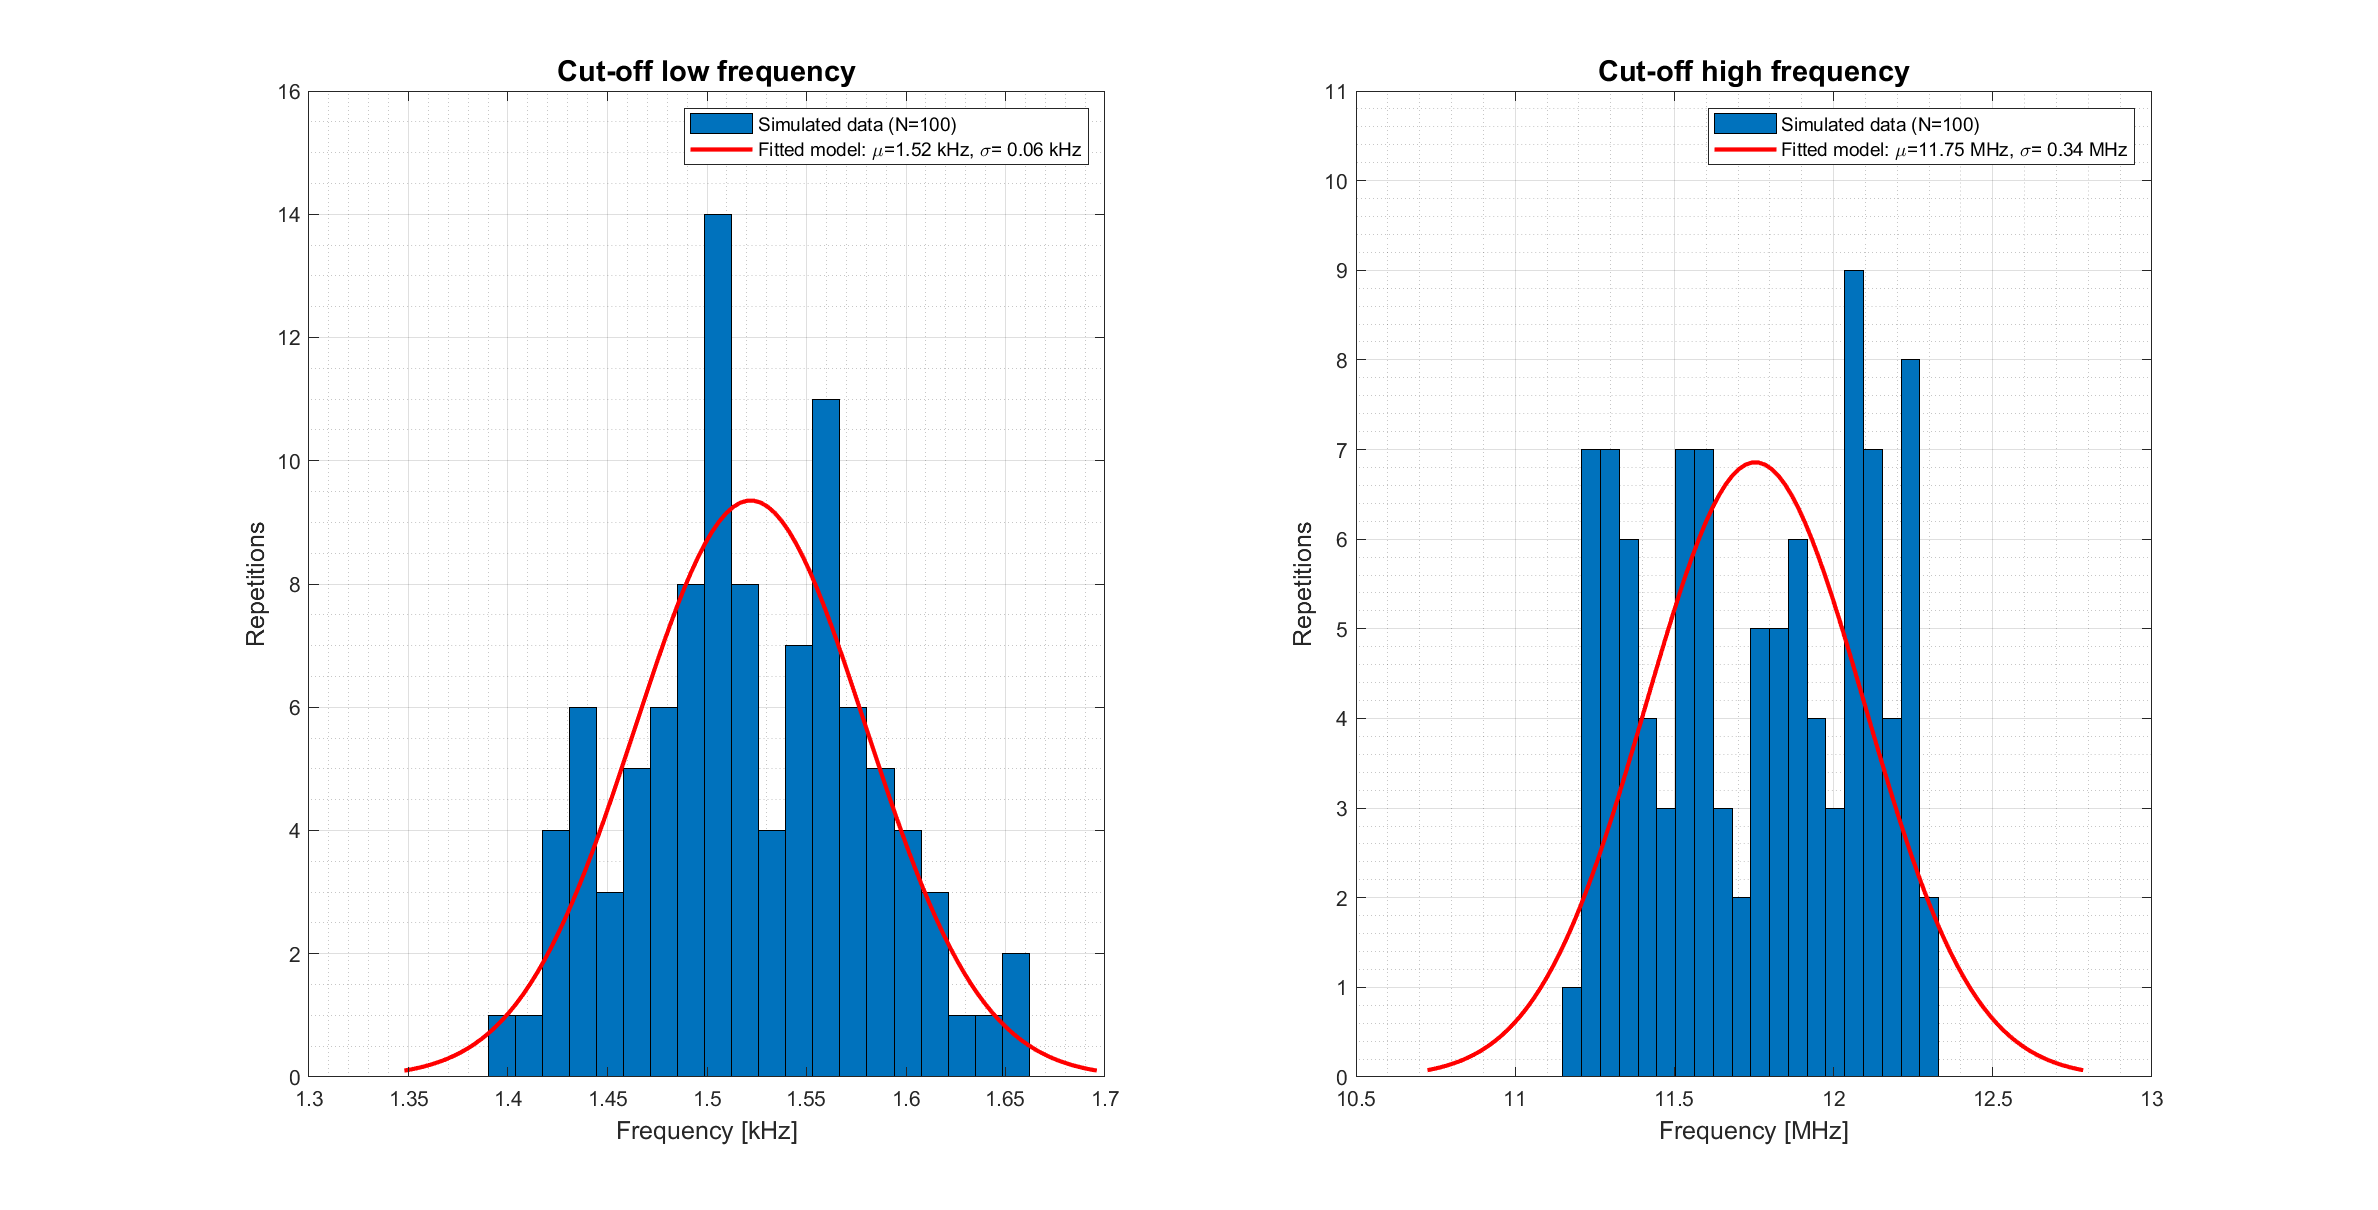
\includegraphics[width=\linewidth]{3_simulacion/fig/Hist_tb1_act_100.png}
    \caption{Análisis estadístico de los lugares de los polos de bajas y altas frecuencias con carga activa, banco de pruebas 1}
\end{figure}

\begin{figure}
    \centering
    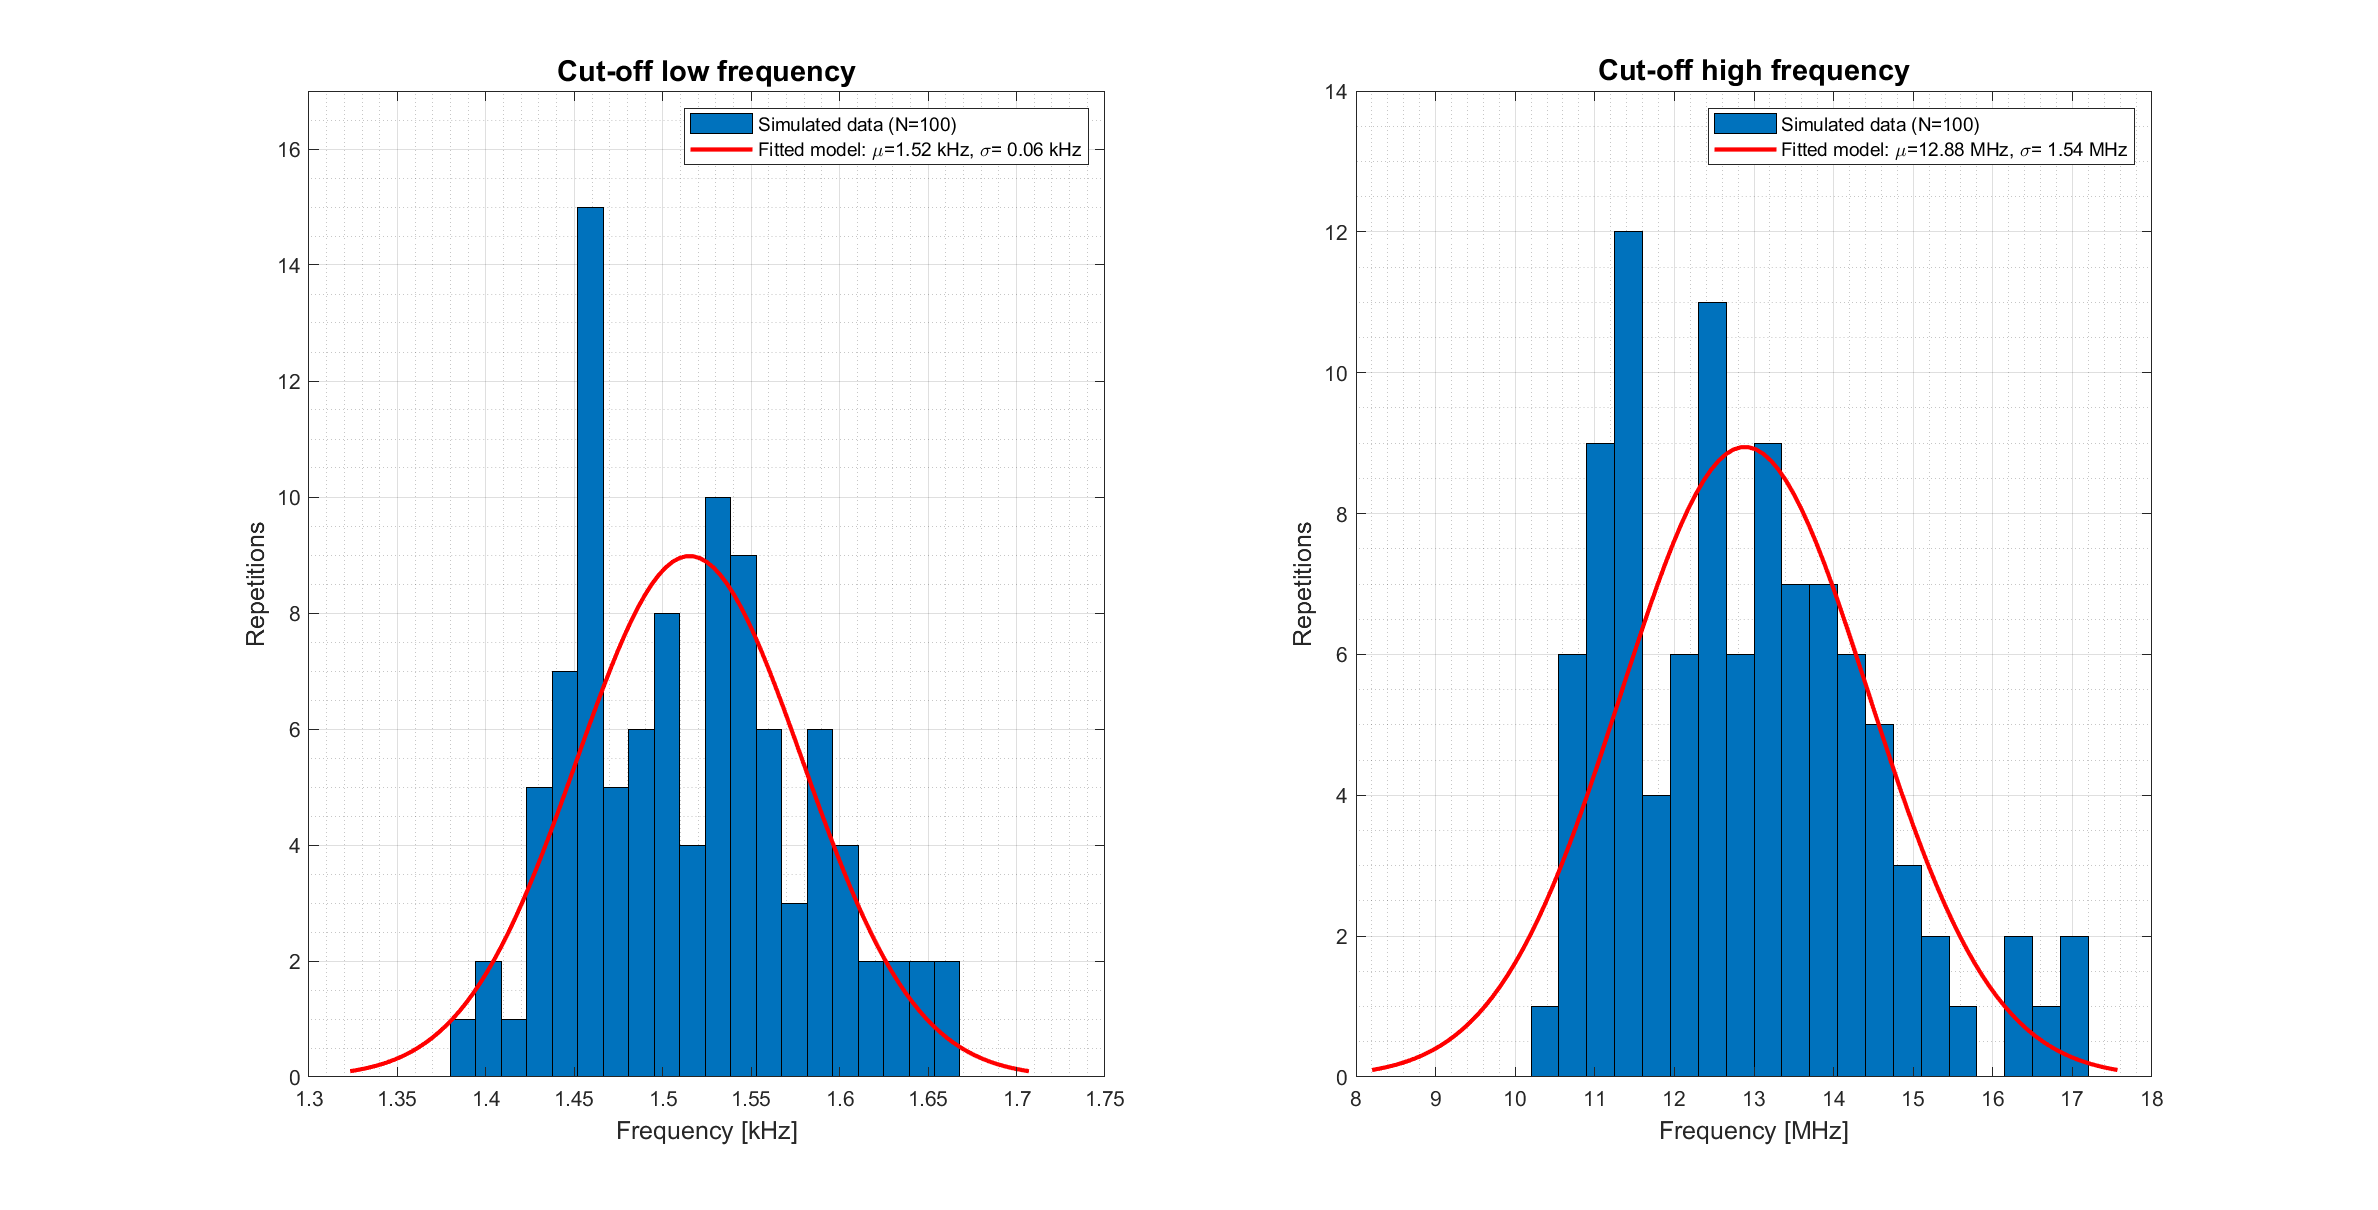
\includegraphics[width=\linewidth]{3_simulacion/fig/Hist_tb2_pas_100.png}
    \caption{Análisis estadístico de los lugares de los polos de bajas y altas frecuencias con carga pasiva, banco de pruebas 2}
\end{figure}

\begin{figure}
    \centering
    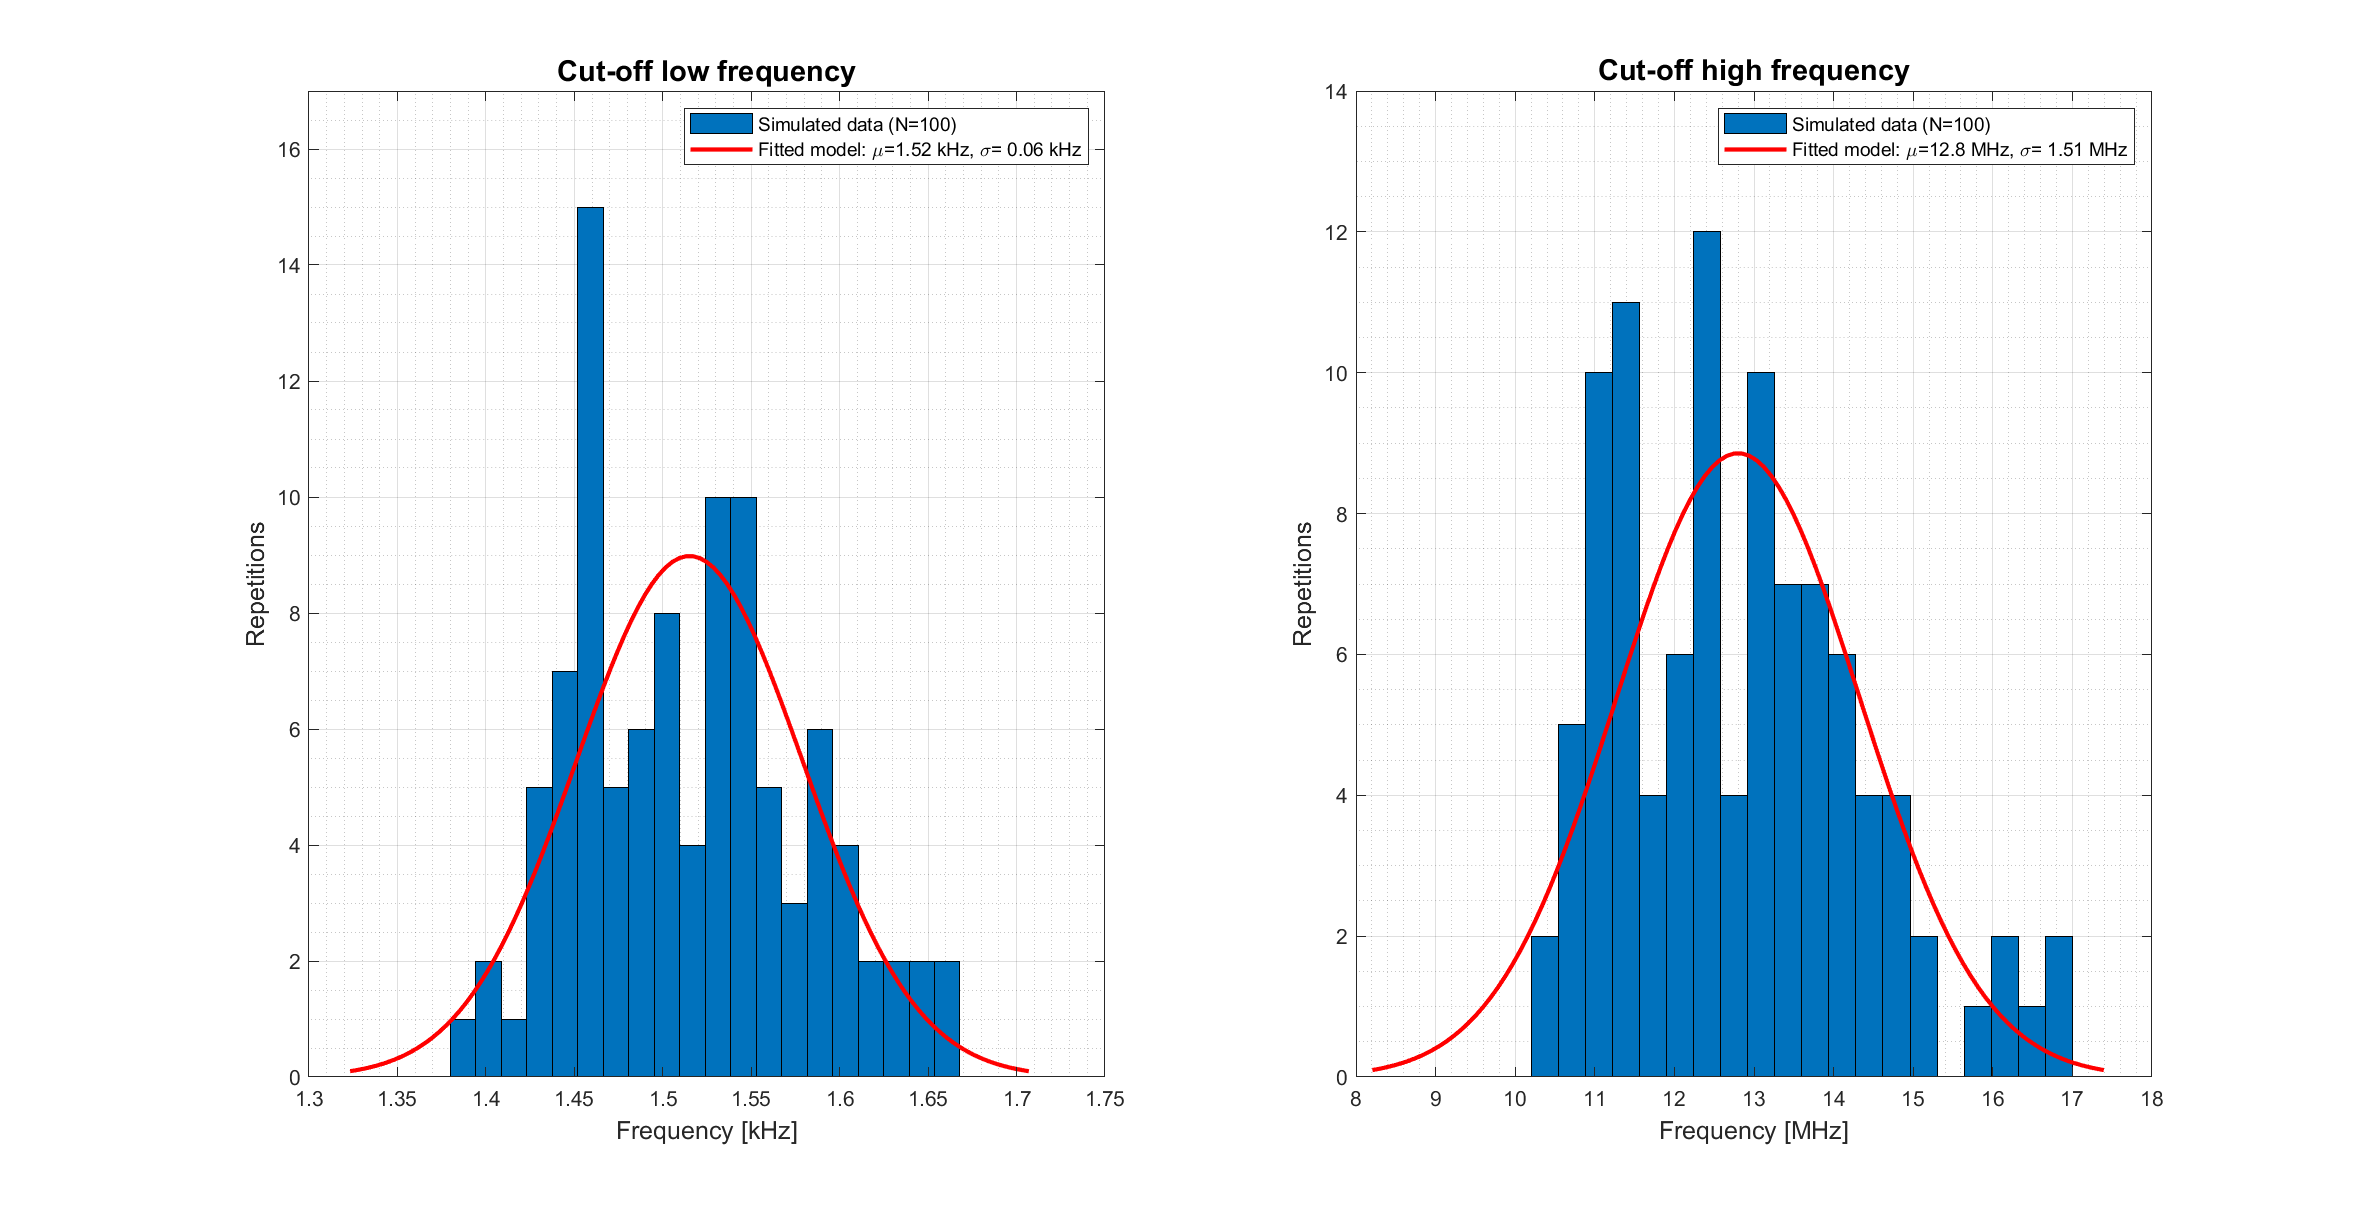
\includegraphics[width=\linewidth]{3_simulacion/fig/Hist_tb2_act_100.png}
    \caption{Análisis estadístico de los lugares de los polos de bajas y altas frecuencias con carga activa, banco de pruebas 2}
\end{figure}
